\documentclass{capstonedoc}

% Document Info
\title{VGA Pixel Buffer}
\date{2016-02-20}
\author{Stephen Just}

\usepackage{tikz-timing}
\usetikztiminglibrary[rising arrows]{clockarrows}

\usepackage{cite}
\usepackage[hyphens]{url}

\usepackage{graphicx}
\graphicspath{ {images/} }

\usepackage{caption}

% Macro from http://nathantypanski.com/blog/2014-10-29-tikz-timing.html
\usepackage{xparse} % NewDocumentCommand, IfValueTF, IFBooleanTF

% Reference a bus.
%
% Usage:
%
%     \busref[3::0]{C/BE}    ->   C/BE[3::0]
%     \busref*{AD}           ->   AD#
%     \busref*[3::0]{C/BE}   ->   C/BE[3::0]#
%
\NewDocumentCommand{\busref}{som}{\texttt{%
#3%
\IfValueTF{#2}{[#2]}{}%
\IfBooleanTF{#1}{\#}{}%
}}

\begin{document}
\maketitle
%Document body

\section{Introduction}

Video output is often a useful addition to interactive projects but typically
there have been many performance limitations with respect to video out on the
DE2. This application note details how it is possible to provide a double
buffered video output without creating large memory bandwidth pressures on
your system's SDRAM that you need to run your application code.

The code package provided with this application note is designed to work on a
DE2 board using any Nios II processor. As with most other applications, the best
performance can be achieved using a faster variant of the processor.

Using the provided code package, you will be able to generate video output
at a resolution of 640x480 with a video refresh rate of 60Hz and use 8-bit
colour. The maximum achievable frame update rate will vary depending on how you
choose to populate the video frame buffers.

\section{Clocking}

Outputting a video signal requires a variety of clocks. Your system clock,
usually running at 50MHz, will be faster than the video pixel clock. For a
640x480@60Hz video signal, a typical pixel clock operates at 25.175MHz.
\cite{VGATiming} The DE2 is not capable of producing that exact frequency,
but it can come close enough with a 25.2MHz clock that can be derived from
the 27MHz oscillator on the board.

To generate a 25.2MHz clock, you can connect the 27MHz clock input to a PLL,
and configure the PLL with a multiplication factor of 14 and a division factor
of 15. In the provided sample code, this is produced by the
\texttt{altpll\_video} Qsys component.

\section{VGA Output}

Altera provides a video output module in the University Program IP collection
to generate the necessary signals to output to the VGA port on the DE2. This
IP is designed to output a 640x480 pixel video signal. The refresh rate of this
VGA signal is determined by the clock you supply to this component. In the
provided sample code, the VGA output block is called
\texttt{video\_vga\_controller\_0}. \cite{UPVideoIP}

The Altera-provided output block has some notable quirks that you should keep
in mind if you want to use it in your own project. Most importantly, it does not
handle incorrectly formatted input in an acceptable way. For example, if you
generate an Avalon-ST data stream with packets of incorrect length, you will
completely lose your video sync and the picture on the screen will appear
incorrectly. The provided \texttt{video\_fb\_streamer\_0} component in the
example code correctly outputs video data for the VGA output block.

In figure~\ref{fig:vgahtiming}, the relationship between a row of pixel data
and the VGA \texttt{hsync} signal is shown. The period surrounding the
\texttt{hsync} pulse where no data is visible is called the horizontal blanking
period. The \texttt{hsync} pulse is preceded by what is called the horizontal
front-porch, and followed by what is called the back-porch. All three of these
components make up the horizontal blanking period.

There is a similar mechanism for vertical timing, where the vertical blanking
period is several multiples of the horizontal timing period long.

\begin{figure}[ht]
\begin{tikztimingtable}[%
    timing/dslope=0.1,
    timing/.style={x=2.5ex,y=2ex},
    x=2.5ex,
    timing/rowdist=3ex,
    timing/name/.style={font=\sffamily\scriptsize}
  ]
  \busref{pixclk}        & 29{c} S 23{c} \\
  \busref{hsync}         & 1h 4l 24h S 23h \\
  \busref{data}          & 13u D{0} D{1} D{2} D{3} D{4} D{5} D{6} D{7} S
                              D{632} D{633} D{634} D{635} D{636} D{637} D{638} D{639} 7u \\
  \extracode
  \begin{pgfonlayer}{background}
    \begin{scope}[semitransparent, semithick]
      \vertlines[darkgray,dotted]{0.5, 1.5,...,26.0}
    \end{scope}
  \end{pgfonlayer}
\end{tikztimingtable}
\caption{VGA Horizontal Timing}
\label{fig:vgahtiming}
\end{figure}

\section{Avalon-ST}

Avalon-ST is the interface used for streaming data between components. This is
the name of the interface that connects the video output components in the
provided example Qsys system.

This bus consists of a data signal, as well as several control signals. The
interface is not bi-directional, and must flow from source to sink.

For video data as we are using it, the Avalon-ST bus must be clocked at the
same rate as the VGA pixel clock: 25.2MHz. Each clock cycle, a pixel is
transferred over the \texttt{data} signal. The first pixel in a frame is
transmitted with the \texttt{startofpacket} control signal asserted. Likewise,
the final pixel in a frame is transmitted with the \texttt{endofpacket} control
signal asserted. The sink will assert \texttt{ready} when it is able to accept
new pixel data. In the case of a VGA video signal, \texttt{ready} is asserted
while pixels are being output to the display, and is de-asserted during the
VGA blanking period.
The \texttt{valid} control signal is asserted by the source when its data is
ready to send. The Altera-provided video blocks expect this signal to always
be asserted.

In figure~\ref{fig:avalonsttiming}, the end of transmitting a video frame is
shown, with the last several pixels being transmitted, and then the first pixel
of the following frame being sent, at which point the VGA controller begins a
blanking period. Note that the next \texttt{data} value must be available before
\texttt{ready} is asserted again.

\begin{figure}[ht]
\begin{tikztimingtable}[%
    timing/dslope=0.1,
    timing/.style={x=5ex,y=2ex},
    x=5ex,
    timing/rowdist=3ex,
    timing/name/.style={font=\sffamily\scriptsize}
  ]
  \busref{clk}           & 22{c} \\
  \busref{ready}         & 1u 1L 8H 1L 1u \\
  \busref{valid}         & 11H \\
  \busref{data[7:0]}     & 1u 1D{$d_{n-7}$} 1D{$d_{n-6}$} 1D{$d_{n-5}$} 1D{$d_{n-4}$} 1D{$d_{n-3}$} 1D{$d_{n-2}$} 1D{$d_{n-1}$} 1D{$d_n$} 1D{$d_0$} 1D{$d_1$} 1u \\
  \busref{startofpacket} & 1u 8L 1H 1L 1u \\
  \busref{endofpacket}   & 1u 7L 1H 2L 1u \\
  \extracode
  \begin{pgfonlayer}{background}
    \begin{scope}[semitransparent, semithick]
      \vertlines[darkgray,dotted]{0.5, 1.5,...,11.0}
    \end{scope}
  \end{pgfonlayer}
\end{tikztimingtable}
\caption{Avalon-ST Timing Diagram}
\label{fig:avalonsttiming}
\end{figure}

\section{Memory}

Altera provides a pixel frame-buffer component similar to the one provided with
this application note in their University Program IP collection, but it was
determined to not be suitable for high performance graphics. The
Altera solution provides two pixel frame-buffers in SDRAM. Either of the buffers
can be output to the VGA controller, with a simple command to swap between which
one is active. The problem that this solution has is that the VGA controller
must always be reading from the SDRAM so that it has pixel data available to
output when it is required. This means that the system processor must compete
with the video output pipeline for access to the SDRAM, which slows down any
drawing operations. If the application code is also running from SDRAM, this
effectively requires the designer to use a variant of the Nios II processor
with a cache.

In the frame-buffer component provided with this application note, a ``live''
frame-buffer exists in SRAM which is continuously read to the video output
pipeline, and a ``working'' frame-buffer exists in SDRAM. A Nios II custom
instruction is provided, \texttt{ci\_frame\_swap\_0}, to trigger a fast copy
from the SDRAM buffer to SRAM.

Because of this arrangement of frame-buffers, it is possible to quickly perform
draw operations to the ``working'' buffer without potentially interrupting the
video output component or without the video output component blocking the
processor.

The copy from SDRAM to SRAM is implemented in such a way that the output video
signal will not experience any video tearing. Tearing occurs when the frame data
changes while the frame is being drawn, so that the user sees parts of two
different versions of the frame at once.

Because part of the SDRAM is dedicated to act as a frame-buffer, it is necessary
that when you write a Nios II application to use this functionality, you modify
the linker settings in your BSP so that the area of memory allocated to your
program does not intersect with that of the frame-buffer. This can be seen in
the provided example code.

\section{Project Setup}

The following sections detail how to configure a project using the provided
video blocks.

\subsection{Qsys}

In Qsys, in addition to the components required for a simple Nios II system, you
must also instantiate a second clock input, a second Avalon ALTPLL, a
\texttt{ci\_frame\_done} custom instruction, a \texttt{video\_fb\_streamer}
component, a \texttt{video\_rgb\_resampler} component, and a
\texttt{video\_vga\_controller} component.

In figure~\ref{fig:qsysclocks}, note that the 50MHz clock is the source of
\texttt{altpll\_sys\_dram}, whereas the 27MHz clock is the source of
\texttt{altpll\_video}. The \texttt{c0} output of \texttt{altpll\_video} is only
connected to the blocks that are part of the video output pipeline, shown in
figure~\ref{fig:qsysvideo}.

\begin{figure}[ht]
  \centering
  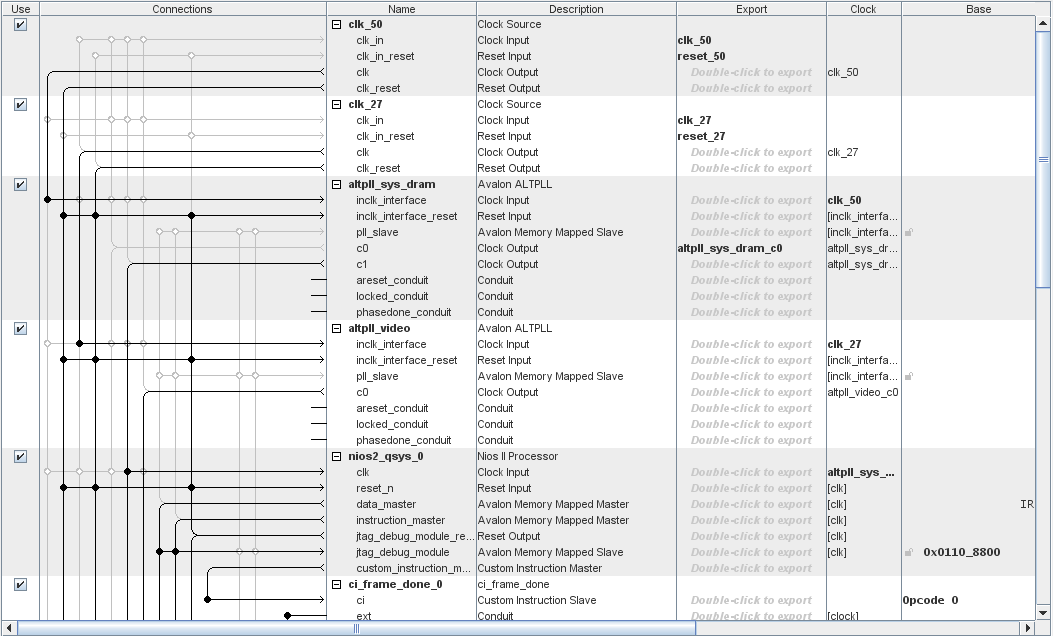
\includegraphics[width=11cm]{qsys_connections_clocks}
  \caption{Clock Connections for Qsys System}
  \label{fig:qsysclocks}
\end{figure}

It is important to note how the each of the video output blocks are connected
to the rest of the system. The \texttt{video\_fb\_streamer} component has two
Avalon-MM Master interfaces on it. Interface \texttt{dma0} must connect to the
SRAM component, while \texttt{dma1} must connect to the SDRAM component. This
allows the streamer component to talk to both memories simultaneously.

Another important thing to note is that the conduits of \texttt{ci\_frame\_done}
and \texttt{video\_fb\_streamer} are connected together. This needs to be
present because the custom instruction interfaces directly with the video
streamer.

In addition to these things, it is important that the base memory address for
the SRAM and SDRAM components are locked. When you configure the
\texttt{video\_fb\_streamer} component, you must provide memory addresses for
both the SDRAM and SRAM video buffers. If the memory addresses for your RAM
components changed, then the streamer component would break. With the base
addresses shown in figure~\ref{fig:qsysvideo}, you can configure the
\texttt{video\_fb\_streamer} block as shown in figure~\ref{fig:qsysvidfbcfg}.

\begin{figure}[ht]
  \centering
  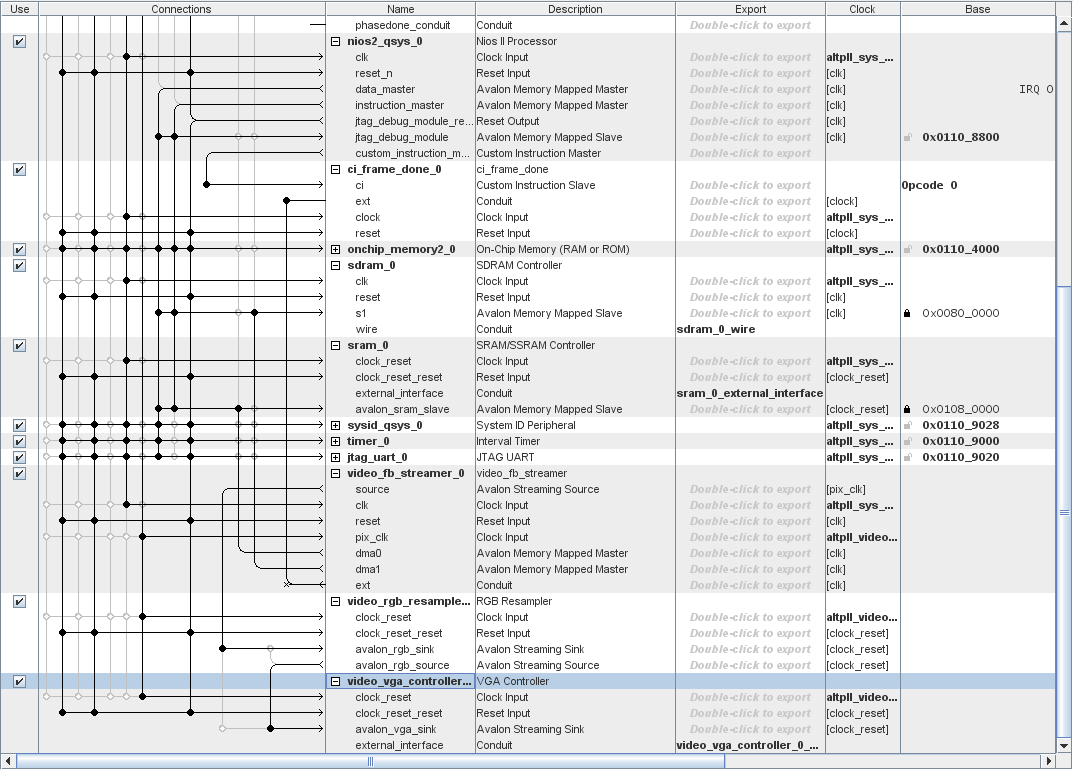
\includegraphics[width=11cm]{qsys_connections_video}
  \caption{Connections for Qsys Video Blocks}
  \label{fig:qsysvideo}
\end{figure}

\begin{figure}[ht]
  \centering
  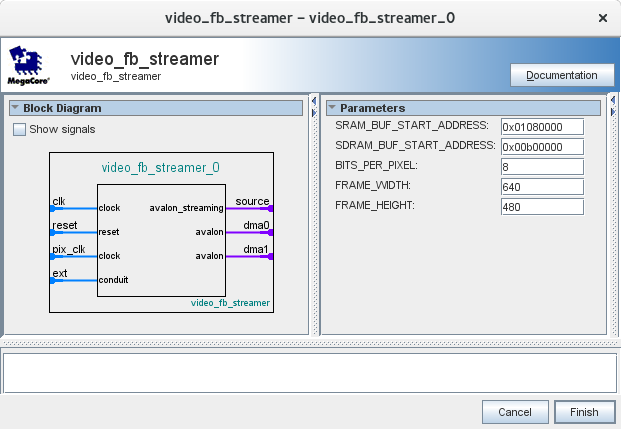
\includegraphics[width=7cm]{qsys_video_fb_streamer}
  \caption{Configuration for \texttt{video\_fb\_streamer}}
  \label{fig:qsysvidfbcfg}
\end{figure}

Finally, the configuration for the \texttt{video\_rgb\_resampler} is shown
in figure~\ref{fig:qsysrgbcfg}. This block must be configured to go from
8-bit colour to 30-bit colour, to match the interfaces of the
\texttt{video\_fb\_streamer} and the \texttt{video\_vga\_controller}.

\begin{figure}[ht]
  \centering
  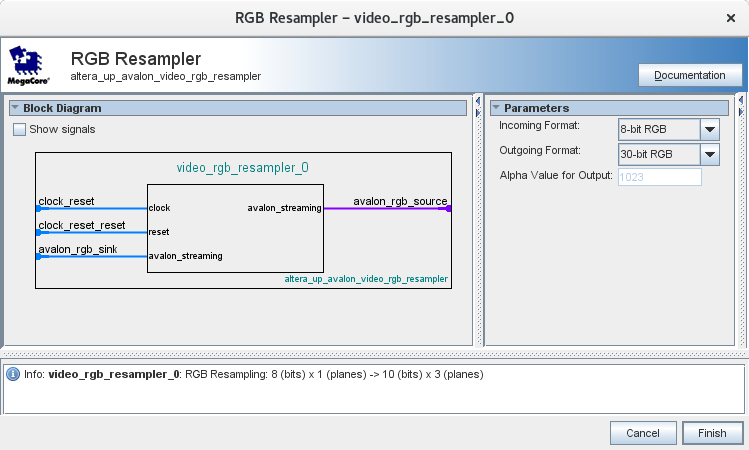
\includegraphics[width=7cm]{qsys_video_rgb_resampler}
  \caption{Configuration for \texttt{video\_rgb\_resampler}}
  \label{fig:qsysrgbcfg}
\end{figure}

\subsection{Quartus}

You can use the Qsys-provided VHDL template to instantiate your system. This
might look something like Listing~\ref{lst:toplevel} below.

\begin{lstlisting}[language=vhdl,caption={Sample Top Level VHDL File},label={lst:toplevel},tabsize=1]
LIBRARY ieee;
USE ieee.std_logic_1164.all;

ENTITY vga_pix_buffer IS
	PORT
	(
		-- Clocks
		CLOCK_50     : in       std_logic;
		CLOCK_27     : in       std_logic;

		-- SDRAM on board
		DRAM_ADDR    : out      std_logic_vector (11 downto 0);
		DRAM_BA_0    : out      std_logic;
		DRAM_BA_1    : out      std_logic;
		DRAM_CAS_N   : out      std_logic;
		DRAM_CKE     : out      std_logic;
		DRAM_CLK     : out      std_logic;
		DRAM_CS_N    : out      std_logic;
		DRAM_DQ      : inout    std_logic_vector (15 downto 0);
		DRAM_LDQM    : out      std_logic;
		DRAM_UDQM    : out      std_logic;
		DRAM_RAS_N   : out      std_logic;
		DRAM_WE_N    : out      std_logic;

		-- SRAM on board
		SRAM_ADDR    : out      std_logic_vector (17 downto 0);
		SRAM_DQ      : inout    std_logic_vector (15 downto 0);
		SRAM_WE_N    : out      std_logic;
		SRAM_OE_N    : out      std_logic;
		SRAM_UB_N    : out      std_logic;
		SRAM_LB_N    : out      std_logic;
		SRAM_CE_N    : out      std_logic;

		-- VGA output
		VGA_R        : out      std_logic_vector (9 downto 0);
		VGA_G        : out      std_logic_vector (9 downto 0);
		VGA_B        : out      std_logic_vector (9 downto 0);
		VGA_CLK      : out      std_logic;
		VGA_BLANK    : out      std_logic;
		VGA_HS       : out      std_logic;
		VGA_VS       : out      std_logic;
		VGA_SYNC     : out      std_logic;

		-- Input buttons
		KEY          : in       std_logic_vector (3 downto 0)
	);
END ENTITY vga_pix_buffer;

ARCHITECTURE arch OF vga_pix_buffer IS

	COMPONENT vga_pix_buffer_system IS
		PORT (
			clk_50_clk                  : in    std_logic           := 'X';
			reset_50_reset_n            : in    std_logic           := 'X';
			clk_27_clk                  : in    std_logic           := 'X';
			reset_27_reset_n            : in    std_logic           := 'X';
			sram_0_external_interface_DQ                    : inout std_logic_vector(15 downto 0) := (others => 'X');
			sram_0_external_interface_ADDR                  : out   std_logic_vector(17 downto 0);
			sram_0_external_interface_LB_N                  : out   std_logic;
			sram_0_external_interface_UB_N                  : out   std_logic;
			sram_0_external_interface_CE_N                  : out   std_logic;
			sram_0_external_interface_OE_N                  : out   std_logic;
			sram_0_external_interface_WE_N                  : out   std_logic;
			video_vga_controller_0_external_interface_CLK   : out   std_logic;
			video_vga_controller_0_external_interface_HS    : out   std_logic;
			video_vga_controller_0_external_interface_VS    : out   std_logic;
			video_vga_controller_0_external_interface_BLANK : out   std_logic;
			video_vga_controller_0_external_interface_SYNC  : out   std_logic;
			video_vga_controller_0_external_interface_R     : out   std_logic_vector(9 downto 0);
			video_vga_controller_0_external_interface_G     : out   std_logic_vector(9 downto 0);
			video_vga_controller_0_external_interface_B     : out   std_logic_vector(9 downto 0);
			sdram_0_wire_addr                               : out   std_logic_vector(11 downto 0);
			sdram_0_wire_ba                                 : out   std_logic_vector(1 downto 0);
			sdram_0_wire_cas_n                              : out   std_logic;
			sdram_0_wire_cke                                : out   std_logic;
			sdram_0_wire_cs_n                               : out   std_logic;
			sdram_0_wire_dq                                 : inout std_logic_vector(15 downto 0) := (others => 'X');
			sdram_0_wire_dqm                                : out   std_logic_vector(1 downto 0);
			sdram_0_wire_ras_n                              : out   std_logic;
			sdram_0_wire_we_n                               : out   std_logic;
			altpll_sys_dram_c0_clk                          : out   std_logic
		);
	END COMPONENT vga_pix_buffer_system;

	-- Signals to interface with DRAM
	SIGNAL BA   : std_logic_vector (1 downto 0);
	SIGNAL DQM  : std_logic_vector (1 downto 0);

BEGIN

	DRAM_BA_1 <= BA(1);
	DRAM_BA_0 <= BA(0);

	DRAM_UDQM <= DQM(1);
	DRAM_LDQM <= DQM(0);

	sys0 : COMPONENT vga_pix_buffer_system
		PORT MAP (
			clk_50_clk                                      => CLOCK_50,
			reset_50_reset_n                                => KEY(0),
			clk_27_clk                                      => CLOCK_27,
			reset_27_reset_n                                => KEY(0),
			sram_0_external_interface_DQ                    => SRAM_DQ,
			sram_0_external_interface_ADDR                  => SRAM_ADDR,
			sram_0_external_interface_LB_N                  => SRAM_LB_N,
			sram_0_external_interface_UB_N                  => SRAM_UB_N,
			sram_0_external_interface_CE_N                  => SRAM_CE_N,
			sram_0_external_interface_OE_N                  => SRAM_OE_N,
			sram_0_external_interface_WE_N                  => SRAM_WE_N,
			video_vga_controller_0_external_interface_CLK   => VGA_CLK,
			video_vga_controller_0_external_interface_HS    => VGA_HS,
			video_vga_controller_0_external_interface_VS    => VGA_VS,
			video_vga_controller_0_external_interface_BLANK => VGA_BLANK,
			video_vga_controller_0_external_interface_SYNC  => VGA_SYNC,
			video_vga_controller_0_external_interface_R     => VGA_R,
			video_vga_controller_0_external_interface_G     => VGA_G,
			video_vga_controller_0_external_interface_B     => VGA_B,
			sdram_0_wire_addr                               => DRAM_ADDR,
			sdram_0_wire_ba                                 => BA,
			sdram_0_wire_cas_n                              => DRAM_CAS_N,
			sdram_0_wire_cke                                => DRAM_CKE,
			sdram_0_wire_cs_n                               => DRAM_CS_N,
			sdram_0_wire_dq                                 => DRAM_DQ,
			sdram_0_wire_dqm                                => DQM,
			sdram_0_wire_ras_n                              => DRAM_RAS_N,
			sdram_0_wire_we_n                               => DRAM_WE_N,
			altpll_sys_dram_c0_clk                          => DRAM_CLK
		);

END ARCHITECTURE arch;
\end{lstlisting}

\subsection{Nios II SBT for Eclipse}

When you create a new ``Nios II Application and BSP from Template'' project in
Eclipse, you must manually configure the memory map used in the BSP project.
This configuration is shown in figure~\ref{fig:bspconfig}. In particular note
the definitions for \texttt{sdram\_video\_0} and \texttt{sdram\_sys\_0}. This
must match your planned memory layout. If you compare the memory addresses in
figure~\ref{fig:bspconfig} and the \texttt{SDRAM\_VIDEO\_OFFSET} value in the
sample code in Listing~\ref{lst:movinglinecode}, they should refer to the same
location in memory.

\begin{figure}[ht]
  \centering
  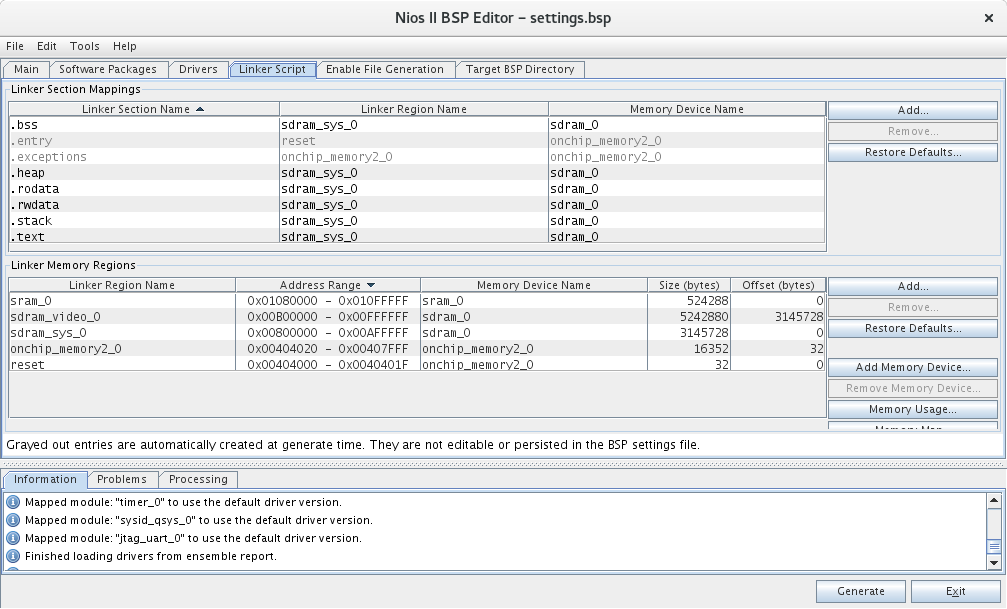
\includegraphics[width=9cm]{bsp_config}
  \caption{BSP Linker Configuration}
  \label{fig:bspconfig}
\end{figure}

\section{Sample Code}

The following code shows how you might draw a simple animation to the video
output.

\begin{lstlisting}[language=c,caption={Sample Program that Generates a Moving Line},label={lst:movinglinecode},tabsize=2]
/* This test program generates a simple pattern to test for tearing.
 *
 * The video pattern consists of a white vertical line that will move
 * from side to side along the frame. If there is tearing, the line
 * will appear broken at some points in time.
 */

#include <io.h>
#include <system.h>

#define SDRAM_VIDEO_OFFSET 0x300000
#define FRAME_WIDTH 640
#define FRAME_HEIGHT 480
#define COLOR_BLACK 0x00
#define COLOR_WHITE 0xFF

int main()
{
	int row = 0;
	int col = 0;

	// Clear the screen
	for (row = 0; row < FRAME_HEIGHT; row++)
	{
		for (col = 0; col < FRAME_WIDTH; col = col + 4)
		{
			IOWR_32DIRECT(SDRAM_0_BASE, SDRAM_VIDEO_OFFSET + row * FRAME_WIDTH + col, COLOR_BLACK);
		}
	}
	ALT_CI_CI_FRAME_DONE_0; // Custom command to trigger frame swap

	// Draw pattern
	unsigned int position = 0;
	while (1)
	{
		for (row = 0; row < FRAME_HEIGHT; row++)
		{
			// Clear previous position of line
			if (position == 0) {
				IOWR_8DIRECT(SDRAM_0_BASE, SDRAM_VIDEO_OFFSET + row * FRAME_WIDTH + FRAME_WIDTH - 8, COLOR_BLACK);
			} else {
				IOWR_8DIRECT(SDRAM_0_BASE, SDRAM_VIDEO_OFFSET + row * FRAME_WIDTH + position - 8, COLOR_BLACK);
			}
			// Draw new line
			IOWR_8DIRECT(SDRAM_0_BASE, SDRAM_VIDEO_OFFSET + row * FRAME_WIDTH + position, COLOR_WHITE);
		}

		position = (position + 8) % 640;
		ALT_CI_CI_FRAME_DONE_0; // Trigger frame swap
	}

	return 0;
}
\end{lstlisting}

\bibliographystyle{ieeetr}
\bibliography{vga_pix_buffer}

\end{document}
